\begin{frame}
    \frametitle{\problemtitle}
    \begin{description}
        \item<+->[Problem:] Find a permutation of the English alphabet such that the strings are sorted.
        \item<+->[Observation:] Trying all permutations is too slow, but many permutations will be killed early.
        \item<+->[Preparation:] Instead of running over the entire list of words every time, create a graph, \\
            adding edges between the first differing pair of letters of two adjacent words:
    \end{description}
    \only<3->{
    \begin{center}
        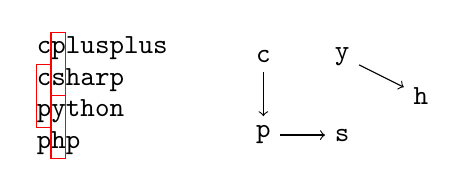
\begin{tikzpicture}
            [->,every edge/.style={->}]
            \node[anchor=west] at (-2,1.1) {\texttt{cplusplus}};
            \node[anchor=west] at (-2,0.7) {\texttt{csharp}};
            \node[anchor=west] at (-2,0.3) {\texttt{python}};
            \node[anchor=west] at (-2,-0.1) {\texttt{php}};

            \draw<3>[draw=red] (-2cm+2.0ex,0.5) rectangle ++(1.2ex,0.8);
            \draw<4>[draw=red] (-2cm+0.8ex,0.1) rectangle ++(1.2ex,0.8);
            \draw<5>[draw=red] (-2cm+2.0ex,-0.3) rectangle ++(1.2ex,0.8);

            \node (p) at (1,0) {\texttt{p}};
            \node (s) at (2,0) {\texttt{s}};
            \node (c) at (1,1) {\texttt{c}};
            \node (y) at (2,1) {\texttt{y}};
            \node (h) at (3,0.5) {\texttt{h}};

            \draw<3-> (p) -- (s);
            \draw<4-> (c) -- (p);
            \draw<5-> (y) -- (h);
        \end{tikzpicture}
    \end{center}
    }
    \begin{description}
        \item<6->[Solution:] If the graph contains a cycle, print ``\texttt{impossible}''. \\
            Else, print the reverse order of a post-order traversal of the graph.
    \end{description}
    \only<7->\solvestats
\end{frame}
